\documentclass{acm_proc_article-sp}
\usepackage{url}
\usepackage{booktabs}
\usepackage{multirow}
\usepackage{graphicx}
\begin{document}
% --- Author Metadata here ---
%\conferenceinfo{PCSC02}{Manila, Philippines}
%\setpagenumber{50}
%\CopyrightYear{2002} % Allows default copyright year (1999) to be over-ridden - IF NEED BE.
%\crdata{0-12345-67-8/90/01}  % Allows default copyright data (0-89791-88-6/97/05) to be %over-ridden - IF NEED BE.
% --- End of Author Metadata ---
\title{AI201 PA 3 Report\\ Two-Layer Multi-Layer Perceptron for Multi-Class Classification}

\numberofauthors{1}
\author{
\alignauthor John Louis D. Lagramada (2025-22174)\\ % your name and student number
~\\
Date of Submission: March 30, 2025
}
% Define \@copyrightspace if the class omitted it (prevents \maketitle error)
\makeatletter
\@ifundefined{@copyrightspace}{\def\@copyrightspace{}}{}
\makeatother

\maketitle


\section{Introduction}
Artificial neural networks (ANN) are feedforward networks that are inspired biologically by how the human brain processes information. Recent breakthroughs in the convergence of these models allow the ubiquity of these models in various applications. In this study, we will explore the performance of a two-layer multi-layer perceptron (MLP) in a multi-class classification task.

The problem of vanishing and exploding gradients is a common issue that is solved using different activation functions that squashes the net internal activities to a stable range. With this, we will explore how three (3) activation functions i.e. hyperbolic tangent (tanh), leaky rectified linear unit (leaky ReLU), and the logistic function affect the performance and training time of the model. 

We also attempt to find the best model by tuning the hyperparameters. In this paper, we examine the effects of different number of hidden neurons on the performance of the model by examining the training and validation losses.  Our architecture consists of two hidden layers with an input layer of 354 features and an output layer of 8 classes.

\subsection{Artificial Neural Networks}
An artificial neural network (ANN) is a machine learning model that learns from data by minimizing the loss function using an optimization algorithm. It consists of layers of interconnected nodes (neurons) that process information based on its weights and biases. The input layer receives the data (features) and "forward" passes through the network to produce an output (class label). This is accomplished by summing the weighted inputs called the net internal activity $v_j(n)$ and applying an activation function $\varphi$ to introduce non-linearity.
\begin{equation}
    v_j(n) = \sum_{i=0}^p w_{ji}(n)\ y_i(n)
\end{equation}
\begin{equation}
    y_j(n) = \varphi(v_j(n))
\end{equation}
The loss is calculated at the output layer because we are training in a supervised manner. The mean squared error (MSE) is calculated to measure the difference between the predicted output and the actual output.
\begin{equation}
    E(n) = \frac{1}{2} \sum_{j=0}^m e_j^2(n)
\end{equation}
where $e_j(n)$ is the error for the $j$-th output neuron
\begin{equation}
    e_j(n) = d_j(n) - y_j(n)
\end{equation}
This error is then backpropagated through the network to update the weights and biases. The $\eta$ is the learning rate which controls the amount of weight updates. We will investigate its effects on finding the weights that minimizes the loss function.
\begin{equation}
\Delta w_{ji}(n)=\eta\delta_j(n)y_i(n)
\end{equation}
where $\delta_j(n)$ is the local gradient defined as,
\begin{equation}
\delta_j{n} =  \begin{cases}
e_j(n)\varphi'(v_j(n)), & \text{for output neurons} \\
\varphi'(v_j(n))\sum_k\delta_k(n)w_{kj}(n), & \text{for hidden neurons}
\end{cases}
\end{equation}


\subsection{Activation Functions}
Activation functions are used to introduce non-linearity in the artificial neural network. Without it, the network would just be a large or deep linear classifier. Additionally, it promotes numerical stability by squashing the net internal activities to a stable range. In this study, we used three (3) activation functions, the hyperbolic tangent (Eq. 7), the leaky rectified linear unit (Eq. 8), and the logistic function (Eq. 9). Since we are interested also in the derivative of these activation functions with respect to $v_j(n)$ they are also easily differentiable with the values we have from the forward pass.

The tanh activation function bounds the net internal activity to $y_j(n) \in [-1, 1]$.
\begin{equation}
    y = a\tanh{(bv)} \qquad y' = \frac{b}{a}(a - y)(a + y)
\end{equation}

The leaky ReLU activation function allows a small, non-zero gradient when the net internal activity is negative, which helps to prevent the dying ReLU problem.
\begin{equation}
    y = \begin{cases}
v, & \text{if } v > 0 \\
\alpha v, & \text{if } v \leq 0
\end{cases} \qquad y' = \begin{cases}
1, & \text{if } v > 0 \\
\alpha, & \text{if } v \leq 0
\end{cases}
\end{equation}

The logistic function is commonly used at the end of a multi-class classification model to produce a probability distribution over the classes.
\begin{equation}
    y = \frac{1}{1 + e^{-v}} \qquad y' = y(1 - y)
\end{equation}

We will compare how a tanh-tanh-logistic MLP performs against a leaky ReLU-leaky ReLU-logistic MLP in terms of performance and training time with the same hyperparameters.

\subsection{Momentum and Weight Updates}
We will employ the generalized delta rule (momentum) to speed up the training process and to help the model escape local minima. A hyperparameter $\alpha$ is used to control the contribution of the previous weight update to the current weight update. 
\begin{equation}
\Delta w_{ji}(n) = \eta \delta_j(n) y_i(n) + \alpha \Delta w_{ji}(n-1)
\end{equation}
We will investigate how the momentum term affects the training time and model convergence.

\subsection{Synthetic Minority Over-Sampling Technique (SMOTE)}
Imbalanced datasets can lead to biased models that performs better on certain classes while poorly on others. To address this problem, the syntheticc minority over-sampling technique or SMOTE is used to duplicate the minority class within a local neighborhood to create synthetic data points that doesn't introduce additional information, but balances the class distributions. SMOTE is used in this paper to balance the highly imbalanced multi-class dataset to improve the performance across all classes.

\subsection{Classifier Evaluation Metrics}
In determining the performance of our classifier, we tuned the hyperparameters that minimizes the loss function as shown in Eq. 3. We then determine the performance of the classifier using accuracy, precision, recall, F1 score, and Matthews correlation coefficient (MCC). We define these metrics as,
\begin{equation}
    \text{Precision} = \frac{\text{TP}}{\text{TP} + \text{FP}}
\end{equation}
\begin{equation}
    \text{Recall} = \frac{\text{TP}}{\text{TP} + \text{FN}}
\end{equation}
\begin{equation}
    \text{F1 Score} = 2 \cdot \frac{\text{Precision} \cdot \text{Recall}}{\text{Precision} + \text{Recall}}
\end{equation}
where $TP$ is the number of true positives, $FP$ is the number of false positives, $TN$ is the number of true negatives, and $FN$ is the number of false negatives. We obtain these metrics individually for each class. We then extend the MCC to the multi-class definition,
\begin{equation}
    \text{MCC} = \frac{ c \cdot s - \sum_{k=1}^{K} (t_k \cdot p_k) }{ \sqrt{ \left( s^2 - \sum_{k=1}^{K} t_k^2 \right) \left( s^2 - \sum_{k=1}^{K} p_k^2 \right) } }
\end{equation}

\section{Objectives}
The objectives of this study is to develop a two-layer multi-layer perceptron for multi-class classification and to investigate the effects of different activation functions and hyperparameters on the performance of the model. Specifically, we aim to:
\begin{enumerate}
    \item Investigate the performance of the two-layer multi-layer perceptron in a multi-class classification task.
    \item Determine the effects of different activation functions on model performance and investigate their time complexities.
    \item Analyze the effects of different number of neurons in the hidden layer by hyperparameter tuning.
    \item Finally, analyze the tradeoff between training time and model convergence with different learning rates and momentum terms.

\end{enumerate}

\section{Methodology}
We implemented a two-layer multi-layer perceptron (MLP) for multi-class classification. The architecture consists of an input layer with 354 features, two hidden layers with varying neurons, and an output layer with 8 classes. We used the Tanh and leaky ReLU activation functions for the hidden layers and the Logistic activation function for the output layer. We trained the model using mini-batch gradient descent with the generalized delta rule (momentum) and evaluated the performance using accuracy, precision, recall, F1-score, and Matthews correlation coefficient (MCC). We also analyzed the training and validation losses to determine the effects of different hyperparameters on model performance and training time. To combat data imbalance, this paper used SMOTE to balance the dataset.

\begin{figure}[h]
    \centering
    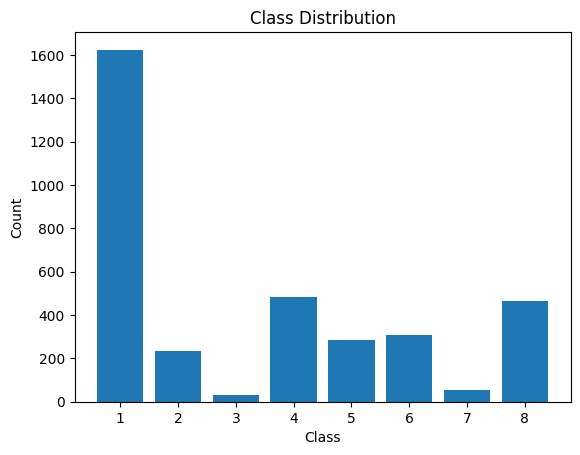
\includegraphics[width=0.225\textwidth]{results/class_imbalance.png}
    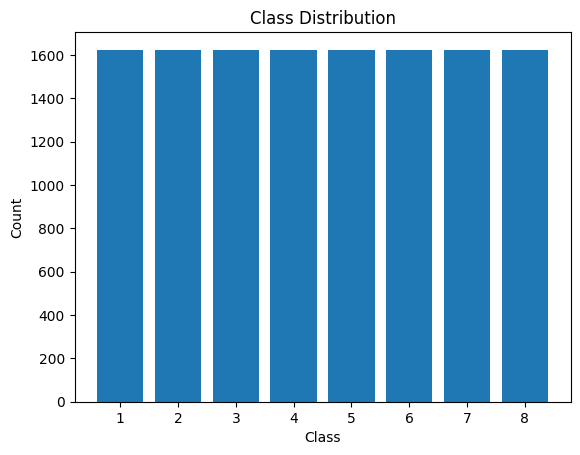
\includegraphics[width=0.225\textwidth]{results/smote.png}
    \caption{Class distributions before and after using SMOTE.}
    \label{fig:f1-scores}
\end{figure}

\subsection{Model Architecture}
The model architecture is a simple two-layer MLP with 354 input nodes, $n + 1$ neurons for the first hidden layer, $m + 1$ neurons for the second hidden layer, and 8 neurons for the output layer. The increment of 1 for the hidden layers is due to a trainable bias term. In the code implementation, the input and output layers can be varied in size. The total number of trainable parameters for this multi-class classification task is,
\begin{equation}
    \theta = 354(m+1) + m(n+1) + 9n
\end{equation}
for a network with 300 neurons for each hidden layer, the total number of parameters are 199208.

\subsection{Mini-batching}
To speed up training, we employed mini-batching since the entire dataset cannot fit in the computer used in training for a batch gradient descent. We determined the best mini-batch size for an x86-64 computer with Ryzen 7 6800U processor and 16GB RAM with 6400 MHz speed. The reported time complexities of the models with different activation functions use the same computer system.

\subsection{Hyperparameter Tuning}
In finding the best classifier model, we performed hyperparameter tuning on the learning rate, momentum term, the activation function used, and the number of neurons in the hidden layer. The set of parameters and hyperparameters used in the study is shown in Table 1.

\begin{table}[h]
\centering
\caption{Ranges of Hyperparameters}
\begin{tabular}{ccccc}
\toprule
Hyperparameter & Values \\
\midrule
input size & 354 \\
output size & 8 \\
a (tanh) & 1.716 \\
b (tanh) & 0.667 \\
a (logistic) & 2.000 \\
$\alpha$ (leaky ReLU) & 0.010 \\
learning rate & [0.005, 0.01, 0.05, 0.1] \\
momentum & [0.1, 0.5, 0.75, 0.9] \\
epochs & 100 \\
perceptrons & [100, 200, 300, 400] \\
mini-batch size & [8, 16, 32, 64, 128] \\
\bottomrule
\end{tabular}
\end{table}

\section{Experimental Results}


\subsection{Tanh MLP vs Leaky ReLU MLP Results}


\subsubsection{Model Performance}
From hereinafter, we will refer to the Tanh-Tanh-Logistic Network as Tanh Network and the Leaky ReLU-Leaky ReLU-Logistic Network as Leaky ReLU network. We plotted the training and validation sum of square errors in Figure 2 of both networks with 100 perceptrons in each hidden layer across 100 epochs. 

\begin{figure}[h]
    \centering
    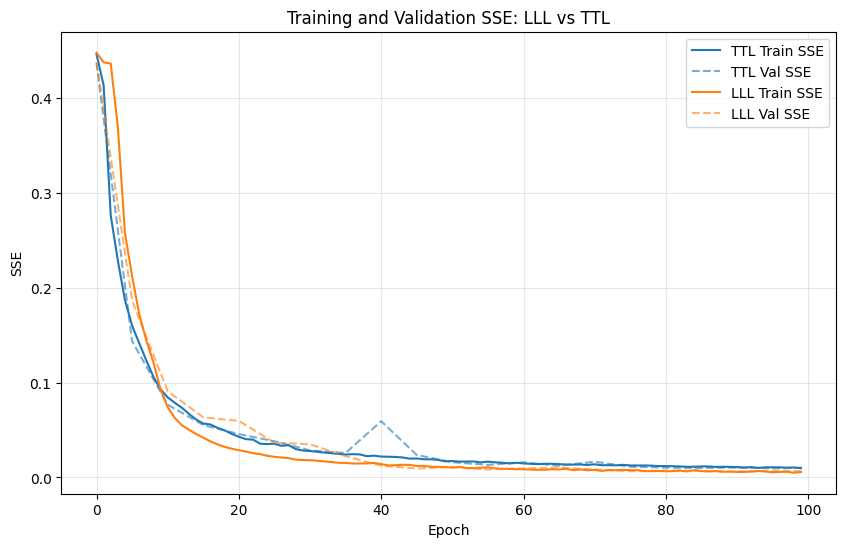
\includegraphics[width=0.475\textwidth]{results/ttl_vs_lll.png}
    \caption{Training and validation errors of Tanh and Leaky ReLU networks.}
    \label{fig:Train-Val-Tanh-ReLU}
\end{figure}

\subsubsection{Training Time}
The average training time per epoch for both Tanh and Leaky ReLU networks are plotted against varying mini-batch sizes to generalize findings. The training times are averaged over 20 epochs for the mini-batch sizes [8, 16, 32, 64, 128]. This also shows the best mini-batch size for subsequent training runs for the computing device, facilitating a much more efficient experimental process as shown in Figure 3.

\begin{figure}[h]
    \centering
    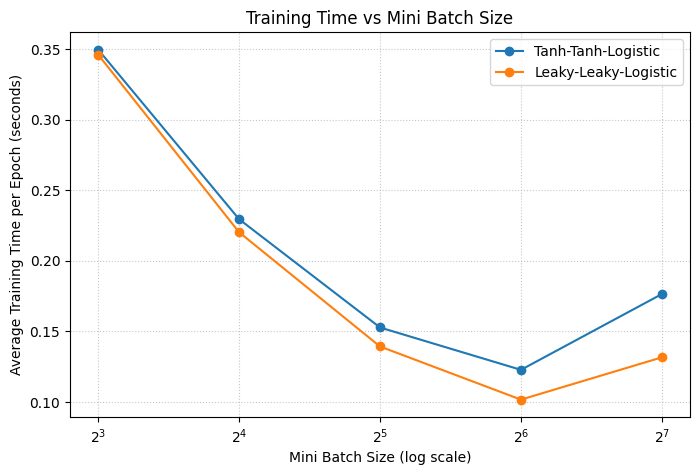
\includegraphics[width=0.475\textwidth]{results/trainingTime_vs_batch.png}
    \caption{Training time comparison of Leaky ReLU and Tanh networks.}
    \label{fig:Training-Time}
\end{figure}


\subsection{Model Convergence}
A model is said to have converged if it reaches a minimum in the loss space. This is achieved by adjusting the weights through gradient descent. The learning rate controls how much the weights are getting updated for each iteration. Momentum, on the other hand, allows faster and more efficient model training by increasing or decreasing weight updates depending on the previous updates.  

\subsubsection{Learning Rate Results}
Figure 4 shows the training and validation errors for different learning rates from [0.005, 0.01, 0.05, 0.1]. From this plot, we can observe how the model diverges as we increase the learning rate.


\begin{figure}[h]
    \centering
    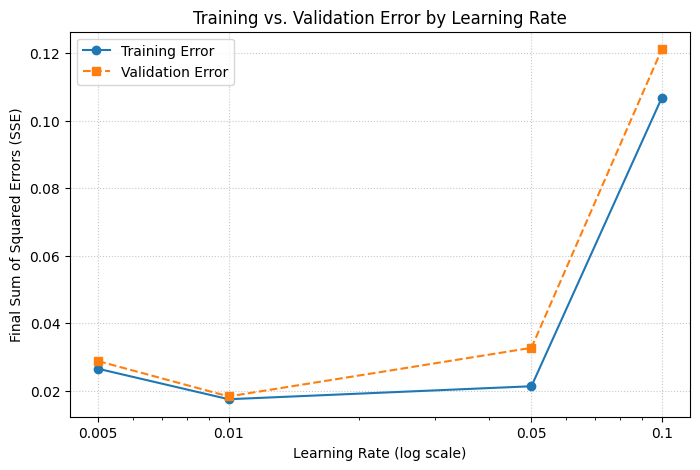
\includegraphics[width=0.475\textwidth]{results/lr_vs_error.png}
    \caption{Training and validation errors for the Tanh network for different learning rates.}
    \label{fig:LR-errors}
\end{figure}

Figure 5 shows the individual plots of the training and validation errors for each learning rate. This shows fluctuations in the error, convergence rate, and training stability. We trained the Tanh network with different learning rates for 50 epochs each.

\begin{figure}[h]
    \centering
    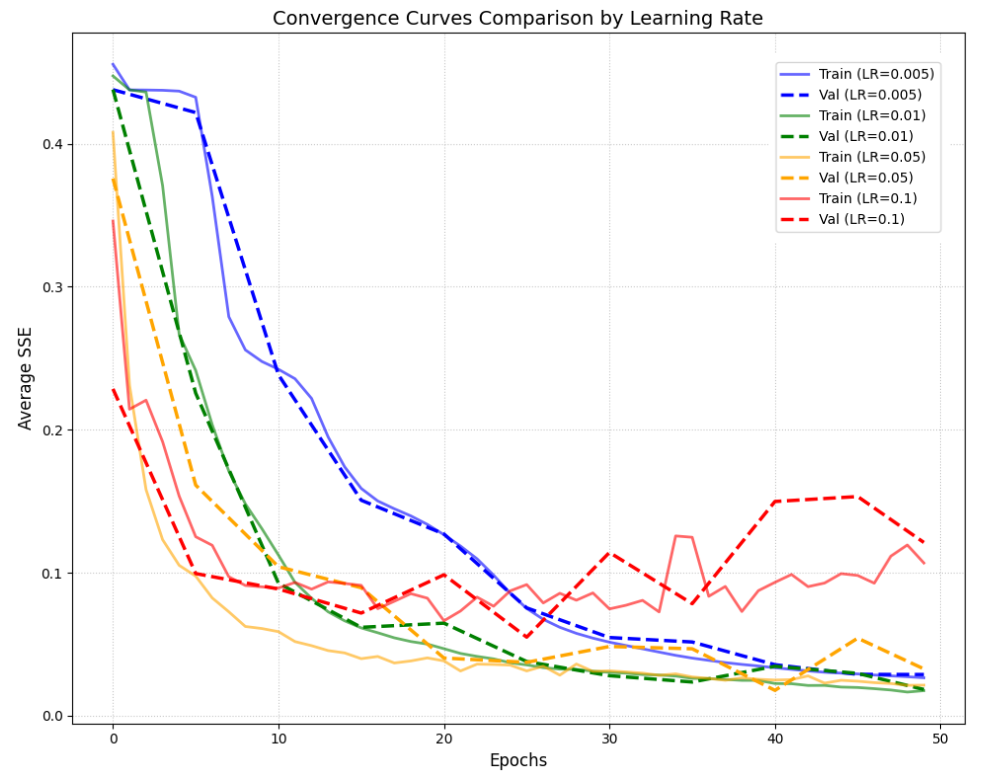
\includegraphics[width=0.475\textwidth]{results/new_error_lr_curves.png}
    \caption{Training and validation error curves for different learning rates across 50 epochs.}
    \label{fig:LR-error-curves}
\end{figure}

\newpage

\subsubsection{Momentum Term Results}
We tested on different momentum terms [0.1, 0.5, 0.75, 0.9] using the Tanh network across 50 epochs. Figure 6 shows the errors per momentum term. From this, we can find a trend of how momentum helps model performance for a given epoch.

\begin{figure}[h]
    \centering
    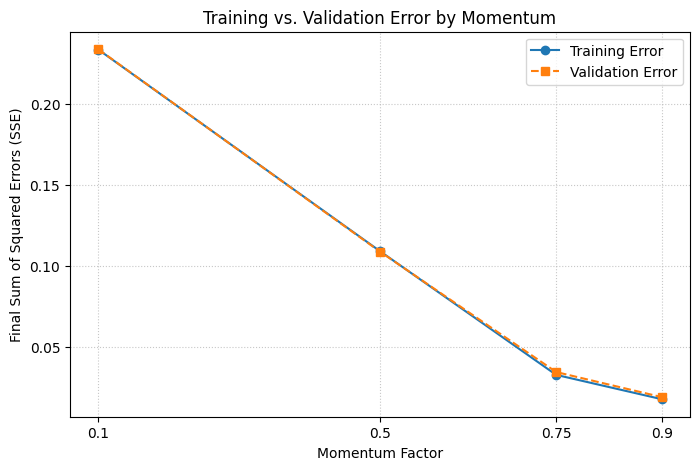
\includegraphics[width=0.475\textwidth]{results/momentum_vs_error.png}
    \caption{Different momentum terms versus training and validation errors.}
    \label{fig:Momentum-errors}
\end{figure}

The individual plots of each model is also plotted in Figure 7 to show trends and characteristics of each curve given different momentum factors.

\begin{figure}[h]
    \centering
    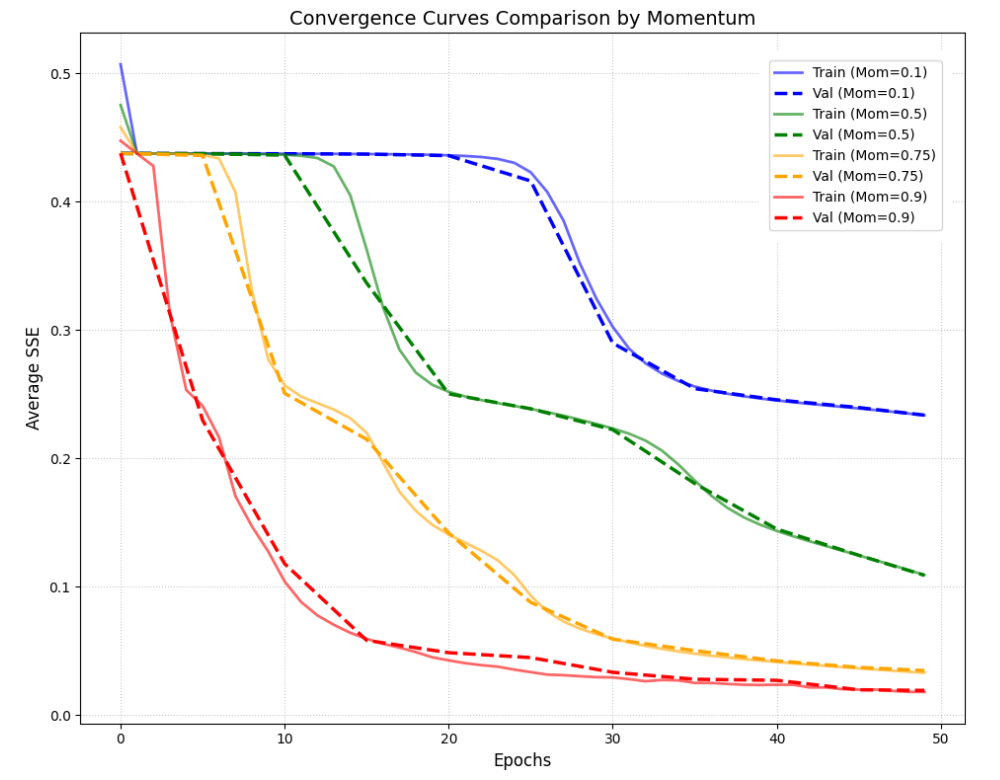
\includegraphics[width=0.475\textwidth]{results/new_error_momentum_curves.png}
    \caption{Training and validation error curves for different momentum terms across 50 epochs.}
    \label{fig:Momentum-error-curves}
\end{figure}

\subsection{Hyperparameter Tuning}
The optimal learning rate, momentum, and mini-batch size hyperparameters are already discovered from the previous experiments. To determine the best model size (by the number of perceptrons in each hidden layer), we experimented on having [100, 200, 300, 400] perceptrons. Each hidden layer has the same number of perceptrons, and so the number of trainable parameters can be simplified to 
\begin{equation}
    \theta = n^2 + 364n + 354
\end{equation}


\subsubsection{Layer Width}
Figure 8 shows how the number of trainable parameters (number of perceptrons per hidden layer) affects the model performance as defined by the training and validation errors.

\begin{figure}[h]
    \centering
    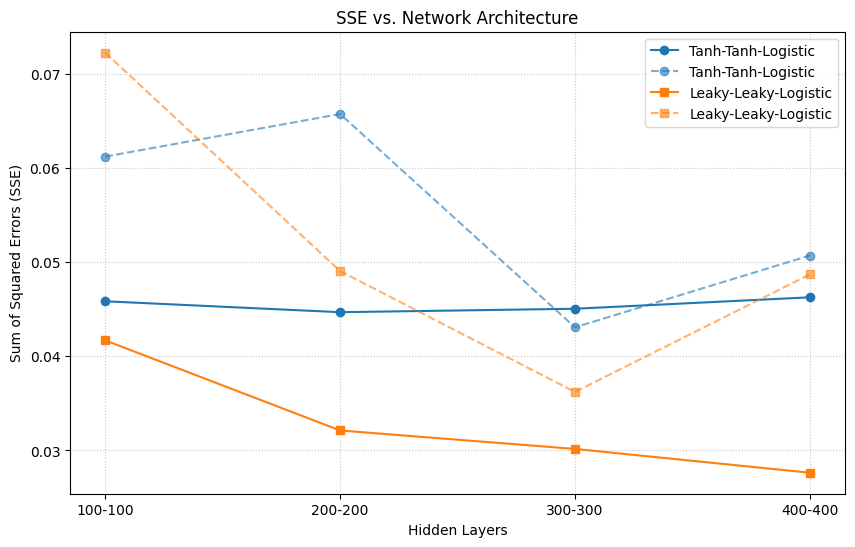
\includegraphics[width=0.475\textwidth]{results/error_vs_layers.png}
    \caption{Training time comparison of Leaky ReLU and Tanh networks.}
    \label{fig:Error-vs-Layers}
\end{figure}

\subsubsection{Best Model Findings}

By determining the optimal hyperparameters, we trained a final best model for both Tanh and Leaky ReLU with the same set of hyperparameters as shown in Table 2. The performance of each model is evaluated using class-wise precision, recall, and F1-score as shown in Table 3 and 4. The Matthew correlation coefficient, accuracy, and number of misclassified labels are shown in Table 5. Lastly, Figure 9 and Figure 10 shows the 8x8 confusion matrix for the Tanh and Leaky ReLU models, respectively.

\begin{table}[h]
\centering
\caption{Optimal Hyperparameters}
\begin{tabular}{ccccc}
\toprule
Hyperparameter & Values \\
\midrule
input size & 354 \\
output size & 8 \\
a (tanh) & 1.716 \\
b (tanh) & 0.667 \\
a (logistic) & 2.000 \\
$\alpha$ (leaky ReLU) & 0.010 \\
learning rate & 0.01 \\
momentum & 0.9 \\
epochs & 100 \\
perceptrons & 300 \\
mini-batch size & 64 \\
\bottomrule
\end{tabular}
\end{table}

\begin{table}[h]
\centering
\caption{Performance Metrics: Tanh-Tanh-Logistic}
\begin{tabular}{cccc}
\toprule
Class & Precision & Recall & F1-Score \\
\midrule
1 & 0.9500 & 0.9794 & 0.9645 \\
2 & 0.9770 & 0.9341 & 0.9551 \\
3 & 0.9510 & 1.0000 & 0.9749 \\
4 & 1.0000 & 0.9533 & 0.9761 \\
5 & 1.0000 & 1.0000 & 1.0000 \\
6 & 0.9208 & 0.9118 & 0.9163 \\
7 & 0.9541 & 1.0000 & 0.9765 \\
8 & 0.9286 & 0.9010 & 0.9146 \\
\bottomrule
\end{tabular}
\end{table}

\begin{table}[h]
\centering
\caption{Performance Metrics: Leaky-Leaky-Logistic}
\begin{tabular}{cccc}
\toprule
Class & Precision & Recall & F1-Score \\
\midrule
1 & 0.9592 & 0.9691 & 0.9641 \\
2 & 0.9890 & 0.9890 & 0.9890 \\
3 & 0.9798 & 1.0000 & 0.9898 \\
4 & 0.9817 & 1.0000 & 0.9907 \\
5 & 1.0000 & 1.0000 & 1.0000 \\
6 & 0.9208 & 0.9118 & 0.9163 \\
7 & 0.9720 & 1.0000 & 0.9858 \\
8 & 0.9681 & 0.9010 & 0.9333 \\
\bottomrule
\end{tabular}
\end{table}

\begin{table}[h]
\centering
\caption{Comparison of Network Performance Metrics}
\begin{tabular}{lcc}
\toprule
Metric & Tanh Network & Leaky Network \\
\midrule
Accuracy & 0.9600 & 0.9712 \\
MCC & 0.9544 & 0.9672 \\
Misclassified & 32 & 23 \\
\bottomrule
\end{tabular}
\end{table}

\begin{figure}[h]
    \centering
    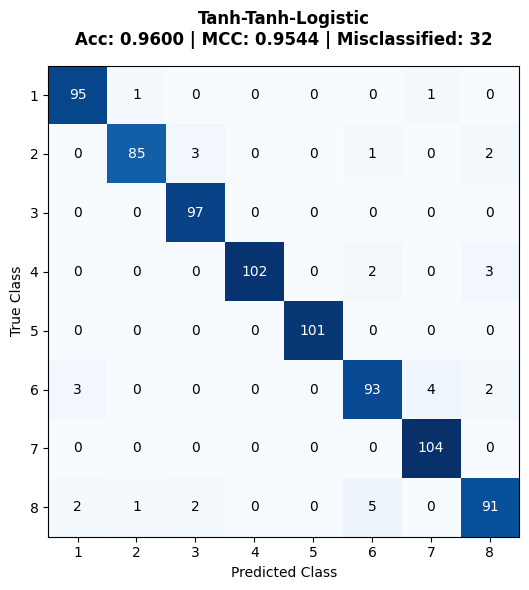
\includegraphics[width=0.475\textwidth]{results/tanh_conf_matrix.png}
    \caption{Confusion matrix of the Tanh Network.}
    \label{fig:Tanh-Conf}
\end{figure}


\begin{figure}[h]
    \centering
    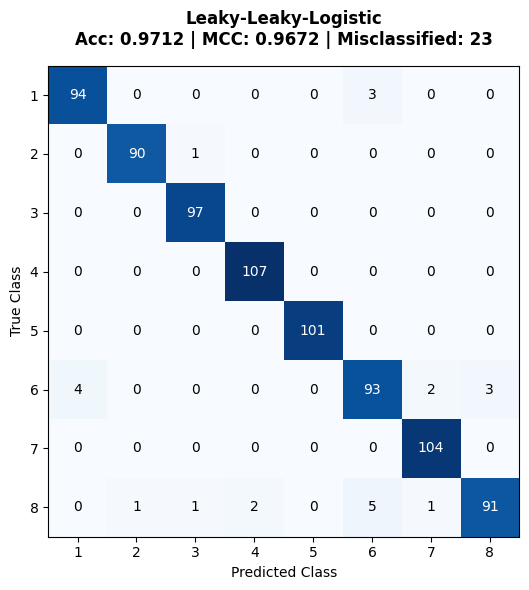
\includegraphics[width=0.475\textwidth]{results/leaky_conf_matrix.png}
    \caption{Confusion matrix of the Leaky ReLU Network.}
    \label{fig:Leaky-Relu-Conf}
\end{figure}




\section{Analysis and Discussion of Results}
In this section, we analyze and discuss the results we obtained from our experiments.

\subsection{Leaky ReLU Network vs Tanh Network}
\subsubsection{Leaky ReLU performs better than Tanh}
Figure 2 shows that the validation and training errors of the Leaky ReLU network are smaller than the Tanh network starting at epoch 10. At epoch 40, the Tanh network also shows a validation error hiccup which it then recovers from. Leaky ReLU shows much more stable training compared to the Tanh network.

The Leaky ReLU network outperforms the Tanh network in accuracy, number of total misclassifications, Matthews correlation coefficient. This means that it performs fairly well for all the classes in the dataset with MCC of 0.9672 over Tanh's 0.9544. The Leaky ReLU network has nine (9) less misclassifications over the Tanh network with a higher accuracy of 0.9712 over Tanh's 0.9600. The confusion matrices shows supports this argument by showing the number of correct classifications and misclassifications by class.
\subsubsection{Leaky ReLU is faster than Tanh}
For all mini-batch sizes tested, the Leaky ReLU network achieved the lower training time compared to the Tanh network. This is because leaky ReLU is just a piecewise function that can easily be implemented with boolean expressions. The Tanh activation function requires exponentiation as shown in Eq. 17 which is costly to compute.
\begin{equation}
    \tanh(x) = \frac{e^{2x}-1}{e^{2x}+1}
\end{equation}
The optimal mini-batch size is 64 data points for the device used in training the models.

~\\

\subsection{Learning Rate}
\subsubsection{High learning rates cause fluctuations}
As shown in Figure 5, high learning rates i.e 0.05 and 0.1 cause fluctuations that are proportional to the learning rates. Figure 4 supports this by showing that further increasing the learning rate causes the model to diverge and produce much higher errors. The fluctuations are attributed to the weights not being adjusted to the local minimum as the weight updates are too large.
\subsubsection{Low learning rates are stable but slow}
The optimal learning rate is 0.01, by lowering it further to 0.005, the model still reaches the a good performant model but it takes a much longer time to do so. This means that the model requires more epochs to achieve the same performance as the optimal learning rate which translates to more computational resources being used.
\subsection{Momentum Terms}
\subsubsection{High momentum escapes local minimum}
A striking observation from Figure 7 shows that the different momentum curves are composed of saddle regions where the average error seems to plateau over several epochs. This can be thought of as local minima, in which the model is stuck thinking that those saddle regions are the global minimum. A high momentum of 0.9 has a curve that doesn't have this saddle region characteristic. Without a momentum term, we may not produce a model that achieved a significantly lower error, because we might think that it is the global minimum ourselves.
\subsubsection{Low momentum cause longer saddle regions}
In addition to our observation in Figure 7, smaller momentum terms have longer saddle regions that can only be observed at further epochs. We theorize that the curve with a momentum term of 0.1 may even reach the global minimum given enough time as it happened to the other momentum terms below 0.9. So far in our experiments, we have only seen two saddle regions, occuring at the start of the training and when the average error is about 0.25. These saddle regions may be specific to the problem, further experimentation is necessary to draw conclusions.
\subsubsection{High momentum is efficient and effective}
A high momentum term helps the model to achieve the lowest loss much faster than lower momentum terms. Additionally, we can see from Figure 6 that the training and validation errors follow a negative trend as we increase the momentum term.

\subsection{Best Models}
\subsubsection{Small models underfit, large models overfit}
As seen in Figure 8, the model that produced the lowest validation errors in both the Tanh and Leaky ReLU networks is the one with 300 perceptrons in both hidden layers. By decreasing the number of hidden layers, the error increases, we can say that the model is \textit{underfitting} the dataset. On the other hand, if we increase the number of perceptrons, the error increases too, we can say that the model is now \textit{overfitting} the dataset. 

Generally, we can see that the models continuously have lower training errors as we increase the number of parameters. This is because the number of trainable parameters is proportional to the information that the model can hold. By increasing it further, we are now memorizing the dataset, by decreasing it, we fail to hold enough information to generalize over the dataset.

\subsubsection{Balanced dataset produce fair results}
Based on the Table 3 and Table 4, the precision, recall, and F1-scores of the different classes are not too far from each other even though the original data distribution is highly imbalanced. This can be said on both models, albeit Leaky ReLU network performs slightly better than the Tanh model. We can say that SMOTE is effective in producing a balanced dataset, and duplicating data points is enough to produce a good performing model without the use of complex synthetic data generation or interpolation methods. From our results, we can also say that a two-layer MLP performs well in multi-class classification task.


\section{Conclusion}
This paper showed that a two-layer MLP can be used as a parametric model for multi-class classification task. Moreover, the Leaky ReLU network performs slightly better than the Tanh network in accuracy, precision, recall, f1-score, and Matthews correlation coefficient (MCC). Leaky ReLU network can also be trained slightly faster than the Tanh network. The two-layer MLP model may overfit or underfit depending on the number of perceptrons in the hidden layers, for this particular task, 300 perceptrons is the optimal number of perceptrons. Both models performed fairly on all classes with the help of synthetic minority oversampling technique or SMOTE.

With hyperparameter tuning, we conclude that the optimal learning rate and momentum term is 0.01 and 0.9, respectively. Our experimentations showed that a high momentum term helped the model escape local minima and reduce saddle region lengths. With that, a high momentum term arrives to the global minimum much faster. The same can be concluded with learning rate, a high learning rate converges much faster. However, a very high learning rate would cause fluctuations as the model cannot reach the minimum due to large weight updates. For small learning rates, the weight updates are small enough to guarantee convergence, but it would take significantly more resources to achieve.


\section{Recommendations}
We recommend experimenting on deeper networks since the implementation of the MLP can be readily extended to any model depth or width. In addition, we recommend experimenting on a grid search approach in finding the best parameters since the hyperparameter tuning methodology we used in this study doesn't account for interactions between the hyperparameters as it will be very costly. We recommend extending this paper on other activation functions such as Gaussian Error Linear Unit (GELU) to determine which activation function produces the best model. Lastly, we recommend investigating if the curve with the momentum term of 0.1 eventually reaches the same error as the one with momentum of 0.9 at further epochs. Lastly, we recommend investigating the effect of a momentum term higher than 0.9 because the trend didn't halt at 0.9 as it may continue to decrease for higher momentum terms.

\begin{thebibliography}{99}

\bibitem{Chawla2002}
Chawla, N. V., Bowyer, K. W., Hall, L. O., \& Kegelmeyer, W. P. (2002). SMOTE: Synthetic minority over-sampling technique. \textit{Journal of Artificial Intelligence Research}, 16, 321--357. arXiv:1106.1813.

\bibitem{Xu2015}
Xu, B., Wang, N., Chen, T., \& Li, M. (2015). Empirical evaluation of rectified activations in convolutional network. \textit{arXiv preprint arXiv:1505.00853}.

\bibitem{Stoica2023}
Stoica, P., \& Babu, P. (2023). Pearson-Matthews correlation coefficients for binary and multinary classification and hypothesis testing. \textit{arXiv preprint arXiv:2305.05974}.

\bibitem{D2L2023}
Zhang, A., Lipton, Z. C., Li, M., \& Smola, A. J. (2023). \textit{Dive into Deep Learning}. Cambridge University Press. \url{https://www.d2l.ai}

\end{thebibliography}

\end{document}


